\subsection{Complexity}
\begin{figure*}[t]
\center
\scalebox{0.6}{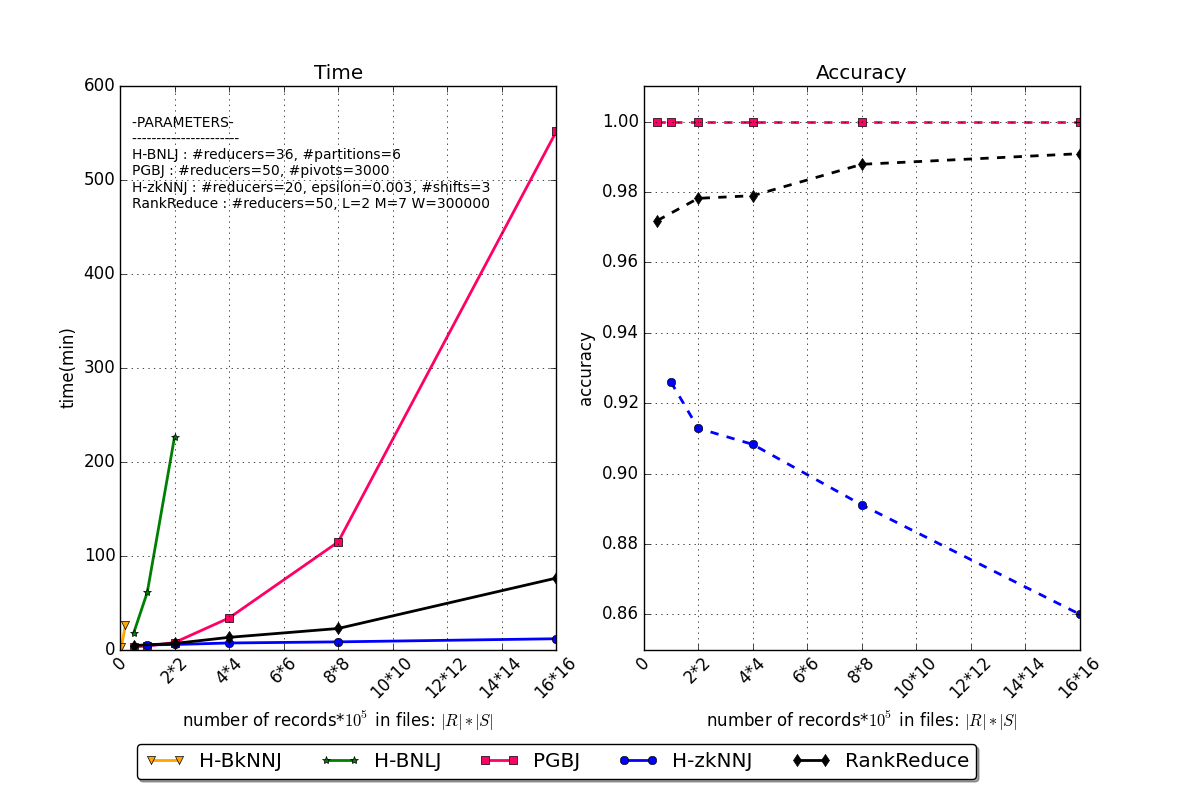
\includegraphics{res/time.png}}
\caption{Completion time and accuracy of knn mapreduce algorithms\label{experiment}}
\end{figure*}
Computational complexity is often used to describe the execution time of an algorithm. When computing kNN with MapReduce, additional factors strongly impact the execution time: 
\begin{itemize}

\item[(1)] \textbf{The number of MapReduce jobs:} Starting a job (whether in 
Hadoop\cite{Jiang:2010:PMI:1920841.1920903} or any other platform) requires some initialization steps 
such as allocating resources and copying data. Those steps can be very time 
consuming.

\item[(2)] \textbf{The number of Map tasks and Reduce tasks used to calculate kNN$\left(R_i \ltimes S\right)$:} The larger this number is, the more 
information is exchanged through the network during the Shuffle phase. 
Moreover, scheduling a task also incurs an overhead.

\item[(3)] \textbf{The number of distances to compute and to sort for each object $r_i$:} Sorting is a dominating operation, so the number of elements to be 
sorted also impacts computation time.
\end{itemize} 

%Here, we analyze the previously described systems 

The basic method H-BkNNJ only uses one MapReduce job, and requires  
$n^2$ Map tasks to calculate the distances where $n$ is the number of 
partitions. The complexity of sorting all distances for one  $r_i$ in $R$ is $
\left|S\right| \times log\left|S\right|$. Since $S$ is usually a large 
dataset, this method quickly becomes impracticable.

To overcome this limitation, H-BNLJ or H-BRJ \cite{Zhang:2012:EPK:2247596.2247602} uses 2 MapReduce jobs, again 
with $n^2$ Map tasks to compute the distances. However, using of a second 
job significantly reduces the complexity of sorting  to $\left|n \cdot k
\right| \times log\left|n \cdot k\right|$, where $n$ is the number of 
partitions and $k$ is the number of nearest neighbors 
queried.

PGBJ\cite{Lu:2012:EPK:2336664.2336674} performs a pre-processing phase followed by 2 MapReduce jobs. This method also 
only uses $n$ Map tasks to calculate the distances. Overall, the sorting complexity is reduced to $\left|S_i\right| \times log\left|S_i\right|$. 

H-zkNNJ\cite{Zhang:2012:EPK:2247596.2247602} also begins by a pre-processing phase and uses in total 3 MapReduce jobs in 
exchange for taking only $n$ Map tasks to compute the distances. Moreover, they only take $
\left(r_i, C_i\left(r_i\right)\right)$, that is the candidate neighbors set, into account. Since $C_i\left(r_i\right)$ contains only $2k$ neighbors for each  
$r_i$, the complexity is now reduced to $\left|2 \cdot k\right| \times log\left|2 \cdot k\right|$.